\documentclass[aspectratio=169,11pt]{beamer}

\usetheme[progressbar=frametitle,numbering=fraction]{metropolis}
\usepackage[T1]{fontenc}
\usepackage[utf8]{inputenc}
\usepackage{booktabs}
\usepackage{tikz}
\usetikzlibrary{positioning,arrows.meta}

\definecolor{accent}{HTML}{1F4E79}
\definecolor{soft}{HTML}{EAF2FB}
\definecolor{warm}{HTML}{C0611B}
\definecolor{warmsoft}{HTML}{FDF1E6}
\setbeamercolor{frametitle}{bg=accent}
\setbeamercolor{progress bar}{fg=warm}
\setbeamercolor{alerted text}{fg=warm}

\newcommand{\ui}[1]{\textsf{\textbf{#1}}}
\newcommand{\sid}[1]{\texttt{#1}}

\tikzset{
  box/.style={draw=accent,rounded corners=2pt,fill=soft,minimum width=2.6cm,
              minimum height=0.75cm,font=\sffamily\small,align=center},
  arr/.style={-{Stealth},thick,accent!70},
  ent/.style={draw=accent,fill=soft,rounded corners=1pt,minimum width=2.3cm,
              minimum height=0.48cm,font=\sffamily\scriptsize},
  inh/.style={ent,draw=gray!60,fill=gray!10,text=gray},
  cutent/.style={ent,fill=warmsoft,draw=warm},
}

\title{Thin Film Logbook}
\subtitle{One place for every sample, step, analysis and data file}
\date{\today}
\institute{CTN}

\begin{document}

\maketitle

%---------------------------------------------------------------------
\begin{frame}{Why a logbook?}
  \small
  \begin{columns}[T]
    \column{0.48\textwidth}
    \textbf{Today}
    \begin{itemize}
      \item Paper notebooks and personal spreadsheets
      \item Data files scattered across instrument PCs and USB sticks
      \item ``Which substrate was that? What was the RTA temperature?''
      \item Hard to hand samples over or find a colleague's results
    \end{itemize}
    \column{0.48\textwidth}
    \textbf{With the logbook}
    \begin{itemize}
      \item A unique ID and a full history for each sample
      \item Parameters entered in structured fields, so they're searchable
      \item Photos and raw data attached where they belong
      \item Shared, searchable, exportable to CSV
    \end{itemize}
  \end{columns}
\end{frame}

%---------------------------------------------------------------------
\begin{frame}{How it's organised}
  \centering
  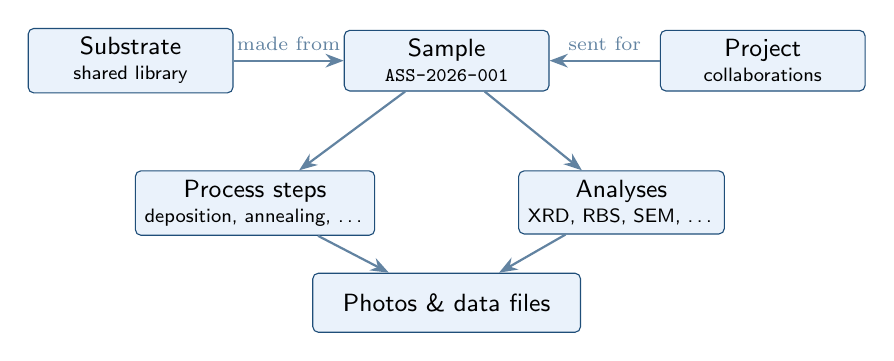
\begin{tikzpicture}
    \node[box] (sub) {Substrate\\[-2pt]\scriptsize shared library};
    \node[box,right=1.4cm of sub] (sam) {Sample\\[-2pt]\scriptsize\texttt{ASS-2026-001}};
    \node[box,right=1.4cm of sam] (prj) {Project\\[-2pt]\scriptsize collaborations};
    \node[box,below left=1.0cm and -0.4cm of sam] (stp) {Process steps\\[-2pt]\scriptsize deposition, annealing, \ldots};
    \node[box,below right=1.0cm and -0.4cm of sam] (ana) {Analyses\\[-2pt]\scriptsize XRD, RBS, SEM, \ldots};
    \node[box,below=2.3cm of sam,minimum width=3.4cm] (att) {Photos \& data files};
    \draw[arr] (sub) -- node[above,font=\scriptsize]{made from} (sam);
    \draw[arr] (prj) -- node[above,font=\scriptsize]{sent for} (sam);
    \draw[arr] (sam) -- (stp);
    \draw[arr] (sam) -- (ana);
    \draw[arr] (stp) -- (att);
    \draw[arr] (ana) -- (att);
  \end{tikzpicture}

  \vspace{0.4cm}
  \small Steps and analyses share one \alert{timeline} per sample.
\end{frame}

%---------------------------------------------------------------------
\begin{frame}{Sample IDs}
  \centering
  \Large\sid{\alert{ASS}-\alert{2026}-\alert{001}-A-2}
  \normalsize

  \vspace{0.3cm}
  {\small initials \quad year \quad counter \quad piece \quad piece of piece}

  \vspace{0.6cm}
  \begin{tabular}{@{}ll@{}}
    \toprule
    \sid{ASS-2026-001}     & ASS's first sample of 2026 \\
    \sid{ASS-2026-001-REF} & a reference piece of it \\
    \sid{UMIN1-2026-001}   & a collaboration sample (project code) \\
    \bottomrule
  \end{tabular}

  \vspace{0.4cm}
  \small Generated automatically and never changed. Use the \ui{Label}
  for your own description.
\end{frame}

%---------------------------------------------------------------------
\begin{frame}{Four kinds of sample}
  \begin{tabular}{@{}lp{9.5cm}@{}}
    \toprule
    \textbf{Thin film}     & a library substrate + dimensions; film material once deposited \\
    \textbf{Bulk}          & a piece of a library substrate; external ID if someone else cut it \\
    \textbf{Commercial}    & description, supplier, batch number, \alert{spec sheet required} \\
    \textbf{Collaboration} & sent by a partner institution: its project, a description, their ID \\
    \bottomrule
  \end{tabular}

  \vspace{0.5cm}
  All of them: optional label and tags, and a researcher (you, or
  someone you create it for).
\end{frame}

%---------------------------------------------------------------------
\begin{frame}{Recording a step or analysis}
  \begin{columns}[T]
    \column{0.5\textwidth}
    \begin{itemize}
      \item Pick the type, and the form shows its fields
      \item \textbf{Where} + \textbf{Equipment}: only the machines at that place
      \item Units built in; \texttt{1e-4} and \texttt{12:30} both work
      \item Dropdowns remember values; \ui{+ Add new\ldots} for a new one
      \item \textbf{Performed by}: whoever ran it can see \& edit that entry
    \end{itemize}
    \column{0.46\textwidth}
    \small
    \textbf{Steps:} Deposition, Annealing (Furnace / RTA), Ion
    Implantation, Lithography, Etching, Cut, Other

    \vspace{0.3cm}
    \textbf{Analyses:} XRD / HRXRD (with modes), XPS, SEM, TEM, RBS, AFM,
    Raman, Optical Microscopy, Hall / 4-probe, Ellipsometry, Profilometry, Other

    \vspace{0.3cm}
    \footnotesize Admins can add types and fields without touching code.
  \end{columns}
\end{frame}

%---------------------------------------------------------------------
\begin{frame}{Photos and data files}
  \begin{columns}[T]
    \column{0.48\textwidth}
    \textbf{\ui{Add photos}}
    \begin{itemize}
      \item Opens the phone camera at the bench
      \item Several at once, or drag onto a card
      \item Resized to $\leq$\,2\,MB, HEIC converted, GPS removed
    \end{itemize}
    \column{0.48\textwidth}
    \textbf{\ui{Attach files}}
    \begin{itemize}
      \item Raw data, \alert{stored exactly as uploaded}
      \item 16-bit TIFFs, \texttt{.raw}, \texttt{.csv}, PDFs, \ldots
      \item Thumbnails on the timeline; one folder per sample on disk
    \end{itemize}
  \end{columns}
\end{frame}

%---------------------------------------------------------------------
\begin{frame}{One run, several samples}
  Same deposition run or same XRD session for several samples?
  \begin{itemize}
    \item Fill in the form once, tick \ui{Also add to other samples}
    \item Each sample gets its own linked copy (``Also on: \ldots'')
    \item Shared photos are stored once, and each sample can get its own data file
    \item Edits can be applied to the whole run, with a warning before
          anything another sample has would be overwritten
  \end{itemize}
\end{frame}

%---------------------------------------------------------------------
\begin{frame}{Cutting a sample into pieces}
  \centering
  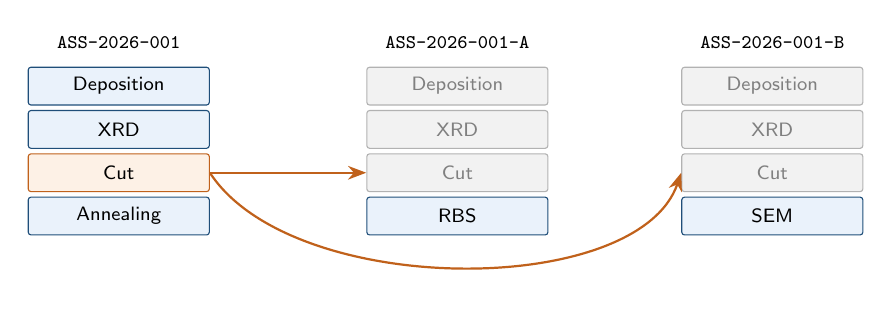
\begin{tikzpicture}
    \node[font=\sffamily\scriptsize\bfseries] at (0,0.55) {\sid{ASS-2026-001}};
    \node[ent] at (0,0) {Deposition};
    \node[ent] at (0,-0.55) {XRD};
    \node[cutent] (p3) at (0,-1.1) {Cut};
    \node[ent] at (0,-1.65) {Annealing};
    \node[font=\sffamily\scriptsize\bfseries] at (4.3,0.55) {\sid{ASS-2026-001-A}};
    \node[inh] at (4.3,0) {Deposition};
    \node[inh] at (4.3,-0.55) {XRD};
    \node[inh] (a3) at (4.3,-1.1) {Cut};
    \node[ent] at (4.3,-1.65) {RBS};
    \node[font=\sffamily\scriptsize\bfseries] at (8.3,0.55) {\sid{ASS-2026-001-B}};
    \node[inh] at (8.3,0) {Deposition};
    \node[inh] at (8.3,-0.55) {XRD};
    \node[inh] (b3) at (8.3,-1.1) {Cut};
    \node[ent] at (8.3,-1.65) {SEM};
    \draw[-{Stealth},thick,warm] (p3.east) -- (a3.west);
    \draw[-{Stealth},thick,warm] (p3.east) .. controls (2.2,-2.7) and (6.6,-2.7) .. (b3.west);
  \end{tikzpicture}

  \vspace{0.3cm}
  \raggedright\small
  \begin{itemize}
    \item Pieces \alert{inherit} the history up to the cut (grey), so a
          correction on the parent reaches every piece
    \item Each piece then has its own entries; pieces can go to other people
    \item Optional reference piece \sid{-REF}
  \end{itemize}
\end{frame}

%---------------------------------------------------------------------
\begin{frame}{Who sees what}
  \begin{columns}[T]
    \column{0.48\textwidth}
    \textbf{Everyone}: each sample's summary
    \begin{itemize}\small
      \item ID, label, type, materials, substrate
      \item tags, techniques used, researcher
    \end{itemize}
    \column{0.48\textwidth}
    \textbf{Details} (parameters, notes, files) are visible to:
    \begin{itemize}\small
      \item the owner and admins
      \item people it's shared with: \ui{View} or \ui{Edit}
      \item for one entry, whoever performed it
    \end{itemize}
  \end{columns}

  \vspace{0.5cm}
  \small Samples can be handed over to another researcher; they confirm
  with \ui{Accept}/\ui{Decline}, and the ID stays the same.
\end{frame}

%---------------------------------------------------------------------
\begin{frame}{Search and export}
  \begin{itemize}
    \item Filter by text, researcher, type, material, technique, tag
    \item Group by researcher, year, type, material, technique, tag, project
    \item \ui{Export results (CSV)}: one row per step/analysis, one column
          per parameter, so it loads straight into Origin, Excel or pandas
    \item Select several samples and share them in one go
  \end{itemize}
\end{frame}

%---------------------------------------------------------------------
\begin{frame}{Also}
  \begin{itemize}
    \item \textbf{Substrate library}: specs and spec sheets entered once, reused
    \item \textbf{Projects}: partner institutions and their samples
    \item \textbf{Suggestions}: report a bug or ask for a field, and admins reply
    \item Portuguese / English, dark mode, works on phones
  \end{itemize}
\end{frame}

%---------------------------------------------------------------------
\begin{frame}{Getting started}
  \begin{enumerate}
    \item Ask an admin for an account
    \item Sign in, set your password, name and \alert{initials}
    \item Create a sample: \ui{New Sample}
    \item Add steps and analyses as you go, with photos from your phone
  \end{enumerate}

  \vspace{0.5cm}
  The user manual (\texttt{docs/manual}) has the details.
\end{frame}

\begin{frame}[standout]
  Questions?
\end{frame}

\end{document}
